\documentclass[a4paper,1pt]{report}
\usepackage[utf8]{inputenc}
\usepackage{amsfonts}
\usepackage{amsthm}
\usepackage{amssymb}
\usepackage{graphicx}
\usepackage{subcaption}
\usepackage{float}

\newtheorem*{pbo}{Principio del Buen Ordenamiento}

\newtheorem*{pim}{Principio de Inducción Matemática}

\newtheorem*{teo}{Teorema}

\newtheorem*{cor}{Corolario}

\newtheorem*{dem}{Demostración}

\newtheorem*{dfn}{Definición}

\newtheorem*{lem}{Lema}

\newtheorem*{prp}{Propiedades}


% Title Page
\title{Conferencia 1 - Introducci\'on a la Teor\'ia de Grafos}
\author{}



\begin{document}
\maketitle

%\begin{abstract}
%\end{abstract}

\begin{dfn}[Grafo]
    Un \textbf{grafo} es un par $G = \langle V, E \rangle $ donde $V$ es un conjunto finito y $E$ es un conjunto de subconjuntos de dos elementos de $V$. A los elementos de $V$ se les llama \textbf{vértices} y a los de $E$ \textbf{aristas}. El conjunto de los vértices se denota $V(G)$ y el de las aristas $E(G)$.
\end{dfn}

\begin{figure}[htb]
\centering
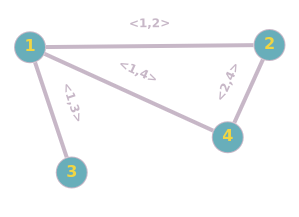
\includegraphics[width=0.3\textwidth]{figures/grafo.png}
\caption{Grafo $G$ con $V(G) = \{1,2,3,4\}$ y $E(G) = \{\{1,2\}, \{1,3\}, \{1,4\}, \{2,4\} \}$}
\end{figure} 

\begin{dfn}[Lazo]
    Un \textbf{lazo} es una arista que tiene un v\'ertice consigo mismo.
\end{dfn}

\begin{dfn}[Arista m\'ultiple]
   Si dos vértices están unidos por más de una arista, estas se llaman \textbf{aristas
    múltiples}.
\end{dfn}

\begin{figure}[h!]
    \centering
    \begin{subfigure}[b]{0.45\textwidth}
    \centering
    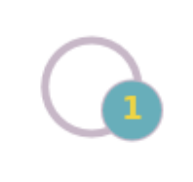
\includegraphics[width=0.3\textwidth]{figures/lazo.png}
    \caption{Ejemplo de lazo}
    \end{subfigure}
    \begin{subfigure}[b]{0.45\textwidth}
        \centering
    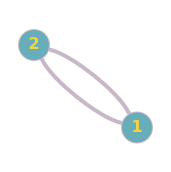
\includegraphics[width=0.4\textwidth]{figures/multiple.png}
    \caption{Ejemplo de arista m\'ultiple}
    \end{subfigure}
\end{figure} 

\begin{dfn}[Multigrafo]
    Un \textbf{multigrafo} es un grafo con aristas múltiples.
\end{dfn}

\begin{dfn}[Pseudografo]
    Un  \textbf{pseudografo} es un multigrafo con lazos.
\end{dfn}

\begin{figure}[h!]
    \centering
    \begin{subfigure}[b]{0.45\textwidth}
    \centering
    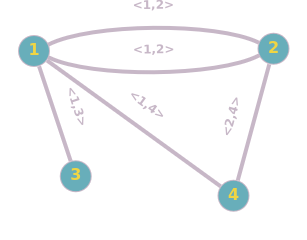
\includegraphics[width=0.5\textwidth]{figures/multigrafo.png}
    \caption{Ejemplo de multigrafo}
    \end{subfigure}
    \begin{subfigure}[b]{0.45\textwidth}
        \centering
    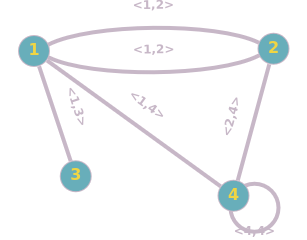
\includegraphics[width=0.5\textwidth]{figures/pseudografo.png}
    \caption{Ejemplo de pseudografo}
    \end{subfigure}
\end{figure} 

\begin{dfn}[Vértices adyacentes]
   Sea $G = \langle V, E \rangle $ un grafo y $v, w \in V(G)$. Se dice que $v$ y $w$ son \textbf{v\'ertices adyacentes} si la arista $e = \{v, w\}\in E(G)$. Se dice que $e$ es incidente a $v$ y $w$.
\end{dfn}

\begin{figure}[H]
    \centering
    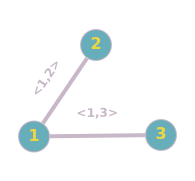
\includegraphics[width=0.2\textwidth]{figures/adyacentes.png}
\caption{Ejemplo de adyacencia, los v\'ertices $1$ y $2$ son adyacentes ya que $\{1,2\} \in E(G)$, mientras que $2$ y $3$ no son adyacentes pues $\{2,3\} \notin E(G)$}
\end{figure}

\begin{dfn}[Grado de un vértice]
    Sea $G = \langle V, E \rangle $ un grafo y $v \in V(G)$. El \textbf{grado de un vértice} $v$ es el número de aristas incidentes a $v$ y se denota como $deg(v)$.
\end{dfn}

\begin{dfn}[Grado máximo y mínimo]
    El \textbf{grado m\'aximo}  de un grafo se denota $\Delta(G) = max\{ deg(v) | v \in V(G)\}$. El \textbf{grado mínimo} de un grafo se denota $\delta(G) = min \{deg(v) | v \in V(G)\}$.
\end{dfn}


\begin{figure}[htb]
    \centering
    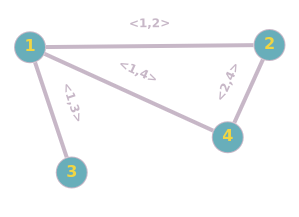
\includegraphics[width=0.3\textwidth]{figures/grafo.png}
    \caption{En este grafo $deg(1) = 3$, $deg(2) = 2$, $deg(4) = 2$ y $deg(3) =1$, adem\'as $\Delta(G) = 3$ y $\delta(G) = 1$}
\end{figure} 
    

\begin{dfn}[Grafo regular]
    Un grafo $G$ es \textbf{regular} si todos sus vértices tienen el mismo grado.
Un grafo $G$  se dice \textbf{regular de grado $k$} si es regular y el grado de cada vértice es $k$.
\end{dfn}

\begin{figure}[htb]
    \centering
    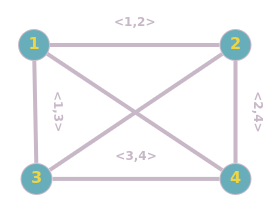
\includegraphics[width=0.2\textwidth]{figures/regular.png}
    \caption{Ejemplo de grafo regular, en este caso es regular de grado 3}
\end{figure} 

\begin{teo}
Sea $G = \langle V, E \rangle$, tal que $|E(G)| = m$, se cumple que la suma de los grados de sus v\'ertices es igual al doble del n\'umero de aristas, es decir: $$\sum_{v \in V(G)} deg(v) = 2 |E(G)| = 2m$$
\end{teo}

\begin{dem}[Via 1: Inducci\'on en $|E(G)|$]\end{dem}

\textit{Caso base $|E(G)| = 0$}: En un grafo sin aristas, el grado de todos sus v\'ertices es $0$, luego $$\sum_{v \in V(G)} deg(v) = 0 = 2 * 0 = 2|E(G)|$$ 

\textit{Hip\'otesis:} Supongamos que para todo grafo $G = \langle V, E \rangle$, tal que $|E(G)| = m$ se cumple que:  $$\sum_{v \in V(G)} deg(v) = 2 |E(G)| = 2m$$

\textit{Demostraci\'on:} Demostremos que para  $G = \langle V, E \rangle$, tal que $|E(G)| = m +1 $ se cumple la propiedad. 

Sea $G' = G - e$, el grafo que se obtiene de remover de $G$ una arista cualquiera, por tanto $V(G') = V(G)$ y $E(G') \subset E(G)$. 

Si le agregamos a $G'$ la arista $e$ que inicialmente hab\'iamos eliminado, esta arista como incide en dos v\'ertices, incrementar\'ia en $2$ la sumatoria de los degrees es decir: $$\sum_{v \in V(G)} deg(v) = \sum_{v \in V(G')} deg(v) +2 $$

Como $|E(G')| = m$, luego por hip\'otesis de inducci\'on se cumple que: $$\sum_{v \in V(G')} deg(v) = 2 |E(G')| = 2m$$

Luego,$$\sum_{v \in V(G)} deg(v) = 2m + 2 = 2(m+1)$$

quedando demostrado el teorema $\blacksquare $.

\begin{dem}[Via 2: Demostraci\'on directa]\end{dem}
Al contar los grados de los vértices se cuentan todas las aristas, pero como cada arista incide en dos v\'ertices, cada arista se cuenta doble en la sumatoria de los grados de los v\'ertices (una vez por cada v\'ertice en el que incide). Luego,
$$\sum_{v \in V(G)} deg(v) = 2 |E(G)| = 2m~ \blacksquare .$$


\begin{cor}
    En todo grafo $G$ es par la cantidad de vértices de grado impar.
\end{cor}

\begin{dem}[Demostraci\'on directa]\end{dem}
Sabemos que la suma de los grados de un grafo es un n\'umero par atendiendo al teorema anterior. Adem\'as podemos separar la sumatoria, en la suma de los v\'ertices de grado par, y la suma de los v\'ertices de grado impar, es decir:

$$\sum_{v \in V(G)} deg(v) = \sum_{v \in V(G) \land deg(v) \equiv 0(2)} deg(v) +  \sum_{v \in V(G) \land deg(v) \equiv 1(2)} deg(v)$$ $$\sum_{v \in V(G)} deg(v) - \sum_{v \in V(G) \land deg(v) \equiv 0(2)} deg(v) =  \sum_{v \in V(G) \land deg(v) \equiv 1(2)} deg(v)$$

Como $\sum_{v \in V(G) \land deg(v) \equiv 0(2)} deg(v)$ es suma t\'erminos pares, el resultado de la sumatoria es par, luego $\sum_{v \in V(G) \land deg(v) \equiv 1(2)} deg(v)$ es tambi\'en un n\'umero par, al ser el resultado de la diferencia entre dos n\'umeros pares.

Como los t\'erminos de $\sum_{v \in V(G) \land deg(v) \equiv 1(2)} deg(v)$ son todos valores impares, la \'unica forma de obtener un resultado par, es sumar una cantidad par de t\'erminos, de donde hay una cantidad par de v\'erticas de grado impar en el grafo $\blacksquare$.

\textbf{Ejemplo:} Sean 9 personas donde cada una le escribe una carta a 3 otras personas. ¿Es posible que todas las personas reciban carta de las mismas personas a quién le enviaron?

Sea un grafo donde los vértices son las personas y las aristas representan que una persona recibió carta de la
persona a la que le envió. Si todos recibieran carta de las personas a las que escribieron, hubieran 9 vértices
de grado 3 y esto no es posible pues en un grafo hay una cantidad par de vértices de grado impar.

\begin{dfn}[Camino]
    Un \textbf{camino} es una secuencia de v\'etices $< v_1,v_2,..., v_k>$, donde $\forall 1\leq i \leq k, ~v_i \in V(G)$, tales que, si $k>1,$ entonces $ \{v_i, v_{i+1}\} \in E(G)$. La longitud del camino es la cantidad de aristas, es decir $k-1$
\end{dfn}

\begin{dfn}[Camino cerrado]
    Un camino es \textbf{cerrado} si su primer v\'ertice es igual al \'ultimo, es decir $v_1 = v_k$.
\end{dfn}

\begin{dfn}[Camino Simple]
    Un camino es \textbf{simple} si no repite v\'ertices.
\end{dfn}

\begin{dfn}[Ciclo]
    Un ciclo es un camino cerrado donde los únicos vértices iguales son el primero y el último y su longitud es mayor o igual que $3$.
\end{dfn}

\begin{figure}[htb]
    \centering
    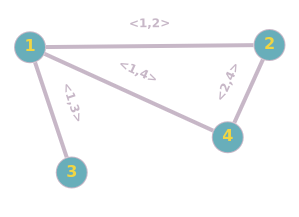
\includegraphics[width=0.3\textwidth]{figures/grafo.png}
    \caption{En este grafo se pueden ilustrar los siguientes ejemplos de camino, camino cerrado, camino simple y ciclo: \\ $C = <1,2,4,1,3>$ es un camino \\ $C = <2,4,1,3,1,2> $ es un camino cerrado  \\ $C =<1,2,4>$ es un camino simple \\ $C =<1,2,4,1>$ es un ciclo}
\end{figure}

\begin{dfn}[Grafo conexo]
    Un grafo es conexo si para todo par de vértices existe un camino que los conecta.
\end{dfn}

\begin{teo}
    Sea $G$ un grafo y $v,w \in V(G), v \neq w$. Si existe un camino que conecta a $v$ con $w$ también existe un camino simple que los une.
\end{teo}

\textbf{Idea para la demostración:} En general, un camino permite repetir vértices, por lo que puede ocurrir esto:

\begin{figure}[H]
    \centering
    
\includegraphics[width=0.4\textwidth]{figures/camino.png}
\end{figure}
La idea es quitar estos “globitos” y lo que queda debajo es el camino simple (no hay vértices repetidos)
buscado.

\begin{dem}[Via 1: Demostraci\'on PBO]\end{dem}
Sea un camino $C = <v =  v_1,v_2,...,v_k =w>$, si $C$ no repite v\'ertices, es un camino simple. En caso contrario, existe al menos un par de v\'ertices repetidos en $C$, es decir  $\exists v_i, v_j \in V(G), i\neq j$ tales que $v_i = v_j$, luego pudiera eliminarse de $C$ el subcamino $<v_{i+1}, v_{i+2}, ..., v_j$, obteni\'endose un $C' = <v =  v_1,... v_i, v_{j+1}, ...,v_k =w >$, (picamos el globito) y $|C'| < |C|$, este proceso lo podemos repetir iterativamente obteniendo cada vez un camino de menor longitud, lo cual provoca un descenso en los enteros positivos
(asociados a las longitudes de los caminos formados) que no puede ser infinito, por PBO. Por eso, este
procedimiento se detiene cuando no hay vértices repetidos resultando un camino simple $\blacksquare$.


\begin{dem}[Via 2: Reducci\'on al Absurdo]\end{dem}
Sea $C$ el menor de todos los caminos que conectan a $v$ con $w$, entonces $C$ es un camino simple. Supongamos que no, entonces $\exists v_i, v_j \in V(G), i\neq j$ tales que $v_i = v_j$, al igual que en la demostraci\'on anterior, al retirar el subcamino (picar el globito) se obtiene un camino $C'$ que es de menor longitud, lo cual es una contradicci\'on puesto que $C$ era el menor de los caminos que conecta a $v$ con $w$, luego $C$ es un camino simple $\blacksquare$.

\begin{dfn}[Distancia]
    Sean $v, w \in V(G)$, se dice que la \textbf{distancia} entre $v$ y $w$ es la longitud del menor camino que los conecta. Se denota como $d(v,w)$
\end{dfn}

\begin{dfn}[Di\'ametro de un grafo]
    El \textbf{di\'ametro de un grafo} $G$ es la mayor de las distancias entre todos los v\'ertices de $V(G)$, es decir $diametro(G) = max\{ d(v,w) | v,w \in V(G)\}$
\end{dfn}

\begin{dfn}[Subgrafo]
    Sea $G_1 = \langle V_1, E_1 \rangle$, $G_2 = \langle V_2, E_2 \rangle$, se dice que $G_2 \subseteq G_1$ si: 
    \begin{itemize}
        \item $V_2 \subseteq V_1$
        \item $E_2 \subseteq E_1$
        \item $\forall e = \{v,w\} \in  E_2 \Rightarrow v,w \in V_2$
    \end{itemize}
\end{dfn}

\begin{figure}[H]
\centering
\begin{subfigure}[b]{0.45\textwidth}
\centering
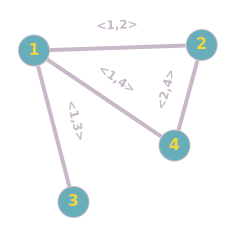
\includegraphics[width=0.5\textwidth]{figures/grafo2.png}
\caption{Grafo $G_1$}
\end{subfigure}
\begin{subfigure}[b]{0.45\textwidth}
    \centering
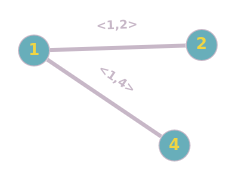
\includegraphics[width=0.5\textwidth]{figures/subgrafo.png}
\caption{Grafo $G_2$}
\end{subfigure}
\caption{Ejemplo donde $G_2 \subseteq G_1$, n\'etese que $V(G_2) \subseteq V(G_1)$ y $E(G_2) \subseteq E(G_1)$}
\end{figure} 


\begin{dfn}[Subgrafo incorporado]
    Sean $G$ y $H$ grafos, se dice que $H$ es \textbf{subgrafo incorporado} (o en expansi\'on  o spanning subgraph) de $G$ si $V(H) = V(G)$.
\end{dfn}

\begin{figure}[H]
\centering
\begin{subfigure}[b]{0.45\textwidth}
\centering
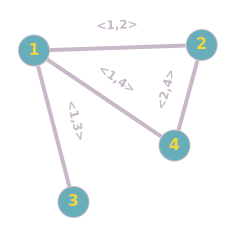
\includegraphics[width=0.5\textwidth]{figures/grafo2.png}
\caption{Grafo $G$}
\end{subfigure}
\begin{subfigure}[b]{0.45\textwidth}
    \centering
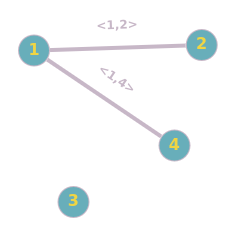
\includegraphics[width=0.5\textwidth]{figures/expansion.png}
\caption{Grafo $H$}
\end{subfigure}
\caption{Ejemplo donde $H$ es subgrafo en expansi\'on de $G$, n\'otese que $V(H) = V(G)$ y $E(H) \subseteq E(G)$}
\end{figure} 

\begin{dfn}[Subgrafo inducido]
    Sea $G$ un grafo y $A \subset V(G)$. El subgrafo de $G$ inducido por $A$, se denota $G[A]$, es aquel que cumple que $V(G[A]) = A$ y $E(G[A]) = \{e \in E(G)| e = \{v,w\} ~ v,w \in A \}$
\end{dfn}
\textbf{Nota:} Un subgrafo inducido es el resultado de tomar los vértices de $A$ con las aristas que tienen relación con
ellos.

\begin{figure}[H]
    \centering
    \begin{subfigure}[b]{0.45\textwidth}
    \centering
    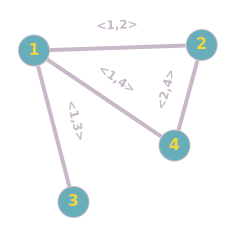
\includegraphics[width=0.5\textwidth]{figures/grafo2.png}
    \caption{Grafo $G$}
    \end{subfigure}
    \begin{subfigure}[b]{0.45\textwidth}
        \centering
    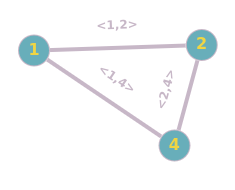
\includegraphics[width=0.5\textwidth]{figures/clique1.png}
    \caption{Grafo $G[A]$ donde $A = \{1,2,4\}$}
    \end{subfigure}
    \caption{Ejemplo donde $G[A]$ es subgrafo inducido por $A$}
    \end{figure} 

\begin{dfn}[Componente Conexa]
    Subgrafo maximal conexo de un grafo
\end{dfn}

\begin{figure}[H]
    \centering
    \begin{subfigure}[b]{0.45\textwidth}
    \centering
    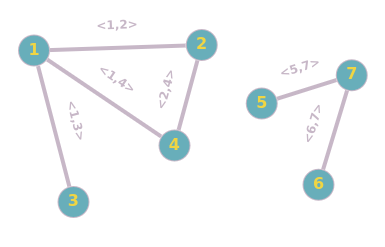
\includegraphics[width=0.5\textwidth]{figures/noConexo.png}
    \caption{Grafo $G$}
    \end{subfigure}
    \begin{subfigure}[b]{0.45\textwidth}
        \centering
    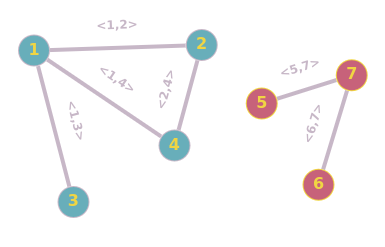
\includegraphics[width=0.5\textwidth]{figures/componentes.png}
    \caption{Componentes conexas de $G$}
    \end{subfigure}
\end{figure} 

\begin{dfn}[Conjunto independiente]
    Un conjunto independiente en un grafo $G$ es un conjunto de vértices
mutuamente no adyacentes (no hay vértices unidos por una arista). Equivale a definir un conjunto $A$ de
vértices donde $G[A]$ no tiene aristas.
\end{dfn}

\begin{figure}[H]
    \centering
    \begin{subfigure}[b]{0.45\textwidth}
    \centering
    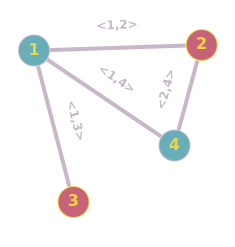
\includegraphics[width=0.5\textwidth]{figures/independiente.png}
    \caption{Grafo $G$}
    \end{subfigure}
    \begin{subfigure}[b]{0.35\textwidth}
        \centering
    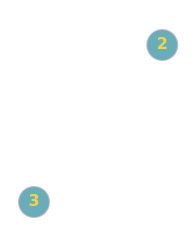
\includegraphics[width=0.5\textwidth]{figures/independiente2.png}
    \caption{Ejemplo de Conjunto independiente de $G$}
    \end{subfigure}
\end{figure} 

\begin{dfn}[Clique]
    Un clique  en un grafo $G$ es un conjunto de vértices mutuamente adyacentes.
\end{dfn}

\begin{figure}[H]
    \centering
    \begin{subfigure}[b]{0.45\textwidth}
    \centering
    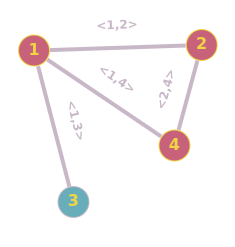
\includegraphics[width=0.5\textwidth]{figures/clique.png}
    \caption{Grafo $G$}
    \end{subfigure}
    \begin{subfigure}[b]{0.45\textwidth}
        \centering
    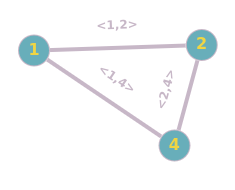
\includegraphics[width=0.5\textwidth]{figures/clique1.png}
    \caption{Ejemplo de Clique de $G$}
    \end{subfigure}
\end{figure} 

\begin{dfn}[N\'umero de independencia]
    El número de independencia de un grafo $G$ es la cardinalidad del conjunto independiente más grande del grafo y se denota $\alpha(G)$.
\end{dfn}

\begin{dfn}[N\'umero de clique]
    El número de clique de un grafo $G$ es la cardinalidad del clique más grande del grafo y se denota $\omega(G)$.
\end{dfn}

\begin{teo}
    En todo grafo, hay al menos dos v\'ertices con el mismo grado
\end{teo}

\begin{dem}[Principio del Palomar]\end{dem}
Sea $G$ un grafo tal que $|V(G)| = n$. Si al menos uno de los v\'ertices es adyacente a todos los dem\'as, los grados del grafo van desde $1$ hasta $n-1$, como hay $n$ v\'ertices y $n-1$ opciones para el valor de sus grados, al menos dos tienen el mismo grado por Principio del Palomar. Si por el contrario, ning\'un v\'ertice se relaciona con todos los otros, entonces los grados del grafo van de $0$ a $n-2$, existiendo de igual modo $n-1$ grados diferentes para $n$ v\'ertices, por palomar, dos v\'ertices al menos tienen el mismo grado $\blacksquare$.


\begin{dfn}[Grafo bipartito]
    Un grafo  $G = \langle V, E \rangle$ es bipartito si $V(G)$ es la unión de dos conjuntos independientes (Si $V(G)$ puede particionarse en dos conjuntos $B$ y $N$ tal que todas las aristas de unen vértices de $B$ y $N$ solamente).
\end{dfn}

\begin{figure}[H]
    \centering
    \begin{subfigure}[b]{0.45\textwidth}
    \centering
    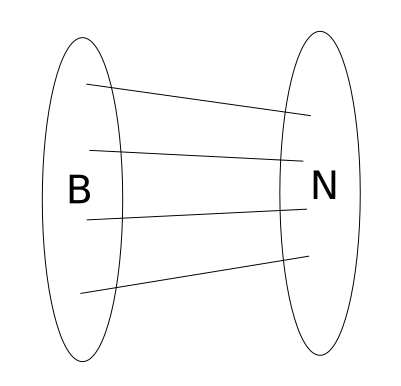
\includegraphics[width=0.5\textwidth]{figures/bipartitoBN.png}
    \caption{Representaci\'on gen\'erica de grafo bipartito}
    \end{subfigure}
    \begin{subfigure}[b]{0.45\textwidth}
        \centering
    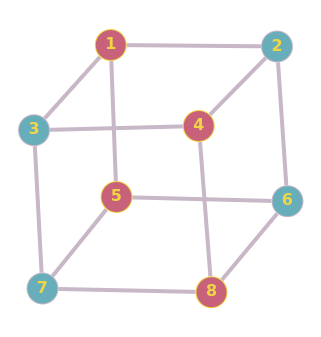
\includegraphics[width=0.5\textwidth]{figures/cubo.png}
    \caption{El cubo como ejemplo de grafo bipartito}
    \end{subfigure}
    \begin{subfigure}[b]{0.45\textwidth}
        \centering
    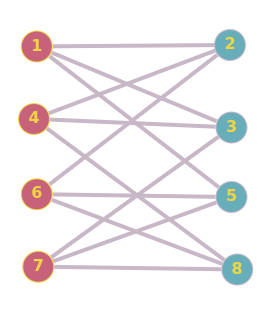
\includegraphics[width=0.5\textwidth]{figures/cuboBipartito.png}
    \caption{El cubo representado en los conjuntos $B$ y $N$}
    \end{subfigure}
\end{figure} 

\begin{dfn}[Grafo Bipartito Completo]
    Un grafo es bipartito completo cuando es bipartito y cada vértice de
un conjunto está unido por una arista a todos los vértices del otro conjunto y se denota
$K_{n1,n2}$, donde $n1$ y $n2$ son las cardinalidades de los conjuntos en que se biparticiona
\end{dfn}
\end{document} 